\chapter{暴力枚举法}


\section{Subsets} %%%%%%%%%%%%%%%%%%%%%%%%%%%%%%
\label{sec:subsets}


\subsubsection{描述}
Given a set of distinct integers, $S$, return all possible subsets.

Note:
\begindot
\item Elements in a subset must be in non-descending order.
\item The solution set must not contain duplicate subsets.
\myenddot

For example, If \code{S = [1,2,3]}, a solution is:
\begin{Code}
[
  [3],
  [1],
  [2],
  [1,2,3],
  [1,3],
  [2,3],
  [1,2],
  []
]
\end{Code}


\subsection{递归}


\subsubsection{增量构造法}
每个元素,都有两种选择,选或者不选。

\begin{Code}
// LeetCode, Subsets
// 增量构造法,深搜,时间复杂度O(2^n),空间复杂度O(n)
class Solution {
public:
    vector<vector<int> > subsets(vector<int> &S) {
        sort(S.begin(), S.end());  // 输出要求有序
        vector<vector<int> > result;
        vector<int> path;
        subsets(S, path, 0, result);
        return result;
    }

private:
    static void subsets(const vector<int> &S, vector<int> &path, int step,
            vector<vector<int> > &result) {
        if (step == S.size()) {
            result.push_back(path);
            return;
        }
        // 不选S[step]
        subsets(S, path, step + 1, result);
        // 选S[step]
        path.push_back(S[step]);
        subsets(S, path, step + 1, result);
        path.pop_back();
    }
};
\end{Code}


\subsubsection{位向量法}
开一个位向量\fn{bool selected[n]},每个元素可以选或者不选。

\begin{Code}
// LeetCode, Subsets
// 位向量法,深搜,时间复杂度O(2^n),空间复杂度O(n)
class Solution {
public:
    vector<vector<int> > subsets(vector<int> &S) {
        sort(S.begin(), S.end());  // 输出要求有序

        vector<vector<int> > result;
        vector<bool> selected(S.size(), false);
        subsets(S, selected, 0, result);
        return result;
    }

private:
    static void subsets(const vector<int> &S, vector<bool> &selected, int step,
            vector<vector<int> > &result) {
        if (step == S.size()) {
            vector<int> subset;
            for (int i = 0; i < S.size(); i++) {
                if (selected[i]) subset.push_back(S[i]);
            }
            result.push_back(subset);
            return;
        }
        // 不选S[step]
        selected[step] = false;
        subsets(S, selected, step + 1, result);
        // 选S[step]
        selected[step] = true;
        subsets(S, selected, step + 1, result);
    }
};
\end{Code}


\subsection{迭代}


\subsubsection{增量构造法}
\begin{Code}
// LeetCode, Subsets
// 迭代版,时间复杂度O(2^n),空间复杂度O(1)
class Solution {
public:
    vector<vector<int> > subsets(vector<int> &S) {
        sort(S.begin(), S.end()); // 输出要求有序
        vector<vector<int> > result(1);
        for (auto elem : S) {
            result.reserve(result.size() * 2);
            auto half = result.begin() + result.size();
            copy(result.begin(), half, back_inserter(result));
            for_each(half, result.end(), [&elem](decltype(result[0]) &e){
                e.push_back(elem);
            });
        }
        return result;
    }
};
\end{Code}


\subsubsection{二进制法}
本方法的前提是:集合的元素不超过int位数。用一个int整数表示位向量,第$i$位为1,则表示选择$S[i]$,为0则不选择。例如\fn{S=\{A,B,C,D\}},则\fn{0110=6}表示子集\fn{\{B,C\}}。

这种方法最巧妙。因为它不仅能生成子集,还能方便的表示集合的并、交、差等集合运算。设两个集合的位向量分别为$B_1$和$B_2$,则$B_1\cup B_2, B_1 \cap B_2, B_1 \triangle B_2$分别对应集合的并、交、对称差。

二进制法,也可以看做是位向量法,只不过更加优化。

\begin{Code}
// LeetCode, Subsets
// 二进制法,时间复杂度O(2^n),空间复杂度O(1)
class Solution {
public:
    vector<vector<int> > subsets(vector<int> &S) {
        sort(S.begin(), S.end()); // 输出要求有序
        vector<vector<int> > result;
        const size_t n = S.size();
        vector<int> v;

        for (size_t i = 0; i < 1 << n; i++) {
            for (size_t j = 0; j < n; j++) {
                if (i & 1 << j) v.push_back(S[j]);
            }
            result.push_back(v);
            v.clear();
        }
        return result;
    }
};
\end{Code}


\subsubsection{相关题目}
\begindot
\item Subsets II,见 \S \ref{sec:subsets-ii}
\myenddot


\section{Subsets II} %%%%%%%%%%%%%%%%%%%%%%%%%%%%%%
\label{sec:subsets-ii}


\subsubsection{描述}
Given a collection of integers that might contain duplicates, $S$, return all possible subsets.

Note:

Elements in a subset must be in non-descending order.
The solution set must not contain duplicate subsets.
For example,
If \fn{S = [1,2,2]}, a solution is:
\begin{Code}
[
  [2],
  [1],
  [1,2,2],
  [2,2],
  [1,2],
  []
]
\end{Code}


\subsubsection{分析}
这题有重复元素,但本质上,跟上一题很类似,上一题中元素没有重复,相当于每个元素只能选0或1次,这里扩充到了每个元素可以选0到若干次而已。


\subsection{递归}


\subsubsection{增量构造法}
\begin{Code}
// LeetCode, Subsets II
// 增量构造法,版本1,时间复杂度O(2^n),空间复杂度O(n)
class Solution {
public:
    vector<vector<int> > subsetsWithDup(vector<int> &S) {
        sort(S.begin(), S.end());  // 必须排序

        vector<vector<int> > result;
        vector<int> path;

        dfs(S, S.begin(), path, result);
        return result;
    }

private:
    static void dfs(const vector<int> &S, vector<int>::iterator start,
            vector<int> &path, vector<vector<int> > &result) {
        result.push_back(path);

        for (auto i = start; i < S.end(); i++) {
            if (i != start && *i == *(i-1)) continue;
            path.push_back(*i);
            dfs(S, i + 1, path, result);
            path.pop_back();
        }
    }
};
\end{Code}

\begin{Code}
// LeetCode, Subsets II
// 增量构造法,版本2,时间复杂度O(2^n),空间复杂度O(n)
class Solution {
public:
    vector<vector<int> > subsetsWithDup(vector<int> &S) {
        vector<vector<int> > result;
        sort(S.begin(), S.end()); // 必须排序

        unordered_map<int, int> count_map; // 记录每个元素的出现次数
        for_each(S.begin(), S.end(), [&count_map](int e) {
            if (count_map.find(e) != count_map.end())
                count_map[e]++;
            else
                count_map[e] = 1;
        });

        // 将map里的pair拷贝到一个vector里
        vector<pair<int, int> > elems;
        for_each(count_map.begin(), count_map.end(),
                [&elems](const pair<int, int> &e) {
                    elems.push_back(e);
                });
        sort(elems.begin(), elems.end());
        vector<int> path; // 中间结果

        subsets(elems, 0, path, result);
        return result;
    }

private:
    static void subsets(const vector<pair<int, int> > &elems,
            size_t step, vector<int> &path, vector<vector<int> > &result) {
        if (step == elems.size()) {
            result.push_back(path);
            return;
        }

        for (int i = 0; i <= elems[step].second; i++) {
            for (int j = 0; j < i; ++j) {
                path.push_back(elems[step].first);
            }
            subsets(elems, step + 1, path, result);
            for (int j = 0; j < i; ++j) {
                path.pop_back();
            }
        }
    }
};
\end{Code}


\subsubsection{位向量法}
\begin{Code}
// LeetCode, Subsets II
// 位向量法,时间复杂度O(2^n),空间复杂度O(n)
class Solution {
public:
    vector<vector<int> > subsetsWithDup(vector<int> &S) {
        vector<vector<int> > result; // 必须排序
        sort(S.begin(), S.end());
        vector<int> count(S.back() - S.front() + 1, 0);
        // 计算所有元素的个数
        for (auto i : S) {
            count[i - S[0]]++;
        }

        // 每个元素选择了多少个
        vector<int> selected(S.back() - S.front() + 1, -1);

        subsets(S, count, selected, 0, result);
        return result;
    }

private:
    static void subsets(const vector<int> &S, vector<int> &count,
            vector<int> &selected, size_t step, vector<vector<int> > &result) {
        if (step == count.size()) {
            vector<int> subset;
            for(size_t i = 0; i < selected.size(); i++) {
                for (int j = 0; j < selected[i]; j++) {
                    subset.push_back(i+S[0]);
                }
            }
            result.push_back(subset);
            return;
        }

        for (int i = 0; i <= count[step]; i++) {
            selected[step] = i;
            subsets(S, count, selected, step + 1, result);
        }
    }
};
\end{Code}


\subsection{迭代}


\subsubsection{增量构造法}
\begin{Code}
// LeetCode, Subsets II
// 增量构造法
// 时间复杂度O(2^n),空间复杂度O(1)
class Solution {
public:
    vector<vector<int> > subsetsWithDup(vector<int> &S) {
        sort(S.begin(), S.end()); // 必须排序
        vector<vector<int> > result(1);

        size_t previous_size = 0;
        for (size_t i = 0; i < S.size(); ++i) {
            const size_t size = result.size();
            for (size_t j = 0; j < size; ++j) {
                if (i == 0 || S[i] != S[i-1] || j >= previous_size) {
                    result.push_back(result[j]);
                    result.back().push_back(S[i]);
                }
            }
            previous_size = size;
        }
        return result;
    }
};
\end{Code}


\subsubsection{二进制法}
\begin{Code}
// LeetCode, Subsets II
// 二进制法,时间复杂度O(2^n),空间复杂度O(1)
class Solution {
public:
    vector<vector<int> > subsetsWithDup(vector<int> &S) {
        sort(S.begin(), S.end()); // 必须排序
        // 用 set 去重,不能用 unordered_set,因为输出要求有序
        set<vector<int> > result;
        const size_t n = S.size();
        vector<int> v;

        for (size_t i = 0; i < 1U << n; ++i) {
            for (size_t j = 0; j < n; ++j) {
                if (i & 1 << j)
                    v.push_back(S[j]);
            }
            result.insert(v);
            v.clear();
        }
        vector<vector<int> > real_result;
        copy(result.begin(), result.end(), back_inserter(real_result));
        return real_result;
    }
};
\end{Code}


\subsubsection{相关题目}
\begindot
\item Subsets,见 \S \ref{sec:subsets}
\myenddot


\section{Permutations} %%%%%%%%%%%%%%%%%%%%%%%%%%%%%%
\label{sec:permutations}


\subsubsection{描述}
Given a collection of numbers, return all possible permutations.

For example,
\fn{[1,2,3]} have the following permutations:
\fn{[1,2,3], [1,3,2], [2,1,3], [2,3,1], [3,1,2]}, and \fn{[3,2,1]}.


\subsection{next_permutation()}
偷懒的做法,可以直接使用\fn{std::next_permutation()}。如果是在OJ网站上,可以用这个API偷个懒;如果是在面试中,面试官肯定会让你重新实现。

\subsubsection{代码}
\begin{Code}
// LeetCode, Permutations
// 时间复杂度O(n!),空间复杂度O(1)
class Solution {
public:
    vector<vector<int> > permute(vector<int> &num) {
        vector<vector<int> > result;
        sort(num.begin(), num.end());

        do {
            result.push_back(num);
        } while(next_permutation(num.begin(), num.end()));
        return result;
    }
};
\end{Code}


\subsection{重新实现next_permutation()}
见第 \S \ref{sec:next-permutation} 节。


\subsubsection{代码}
\begin{Code}
// LeetCode, Permutations
// 重新实现 next_permutation()
// 时间复杂度O(n!),空间复杂度O(1)
class Solution {
public:
    vector<vector<int> > permute(vector<int> &num) {
        vector<vector<int> > result;
        sort(num.begin(), num.end());

        do {
            result.push_back(num);
        // 调用的是 2.1.12 节的 next_permutation()
        // 而不是 std::next_permutation()
        } while(next_permutation(num.begin(), num.end()));
        return result;
    }
};
\end{Code}


\subsection{递归}
本题是求路径本身,求所有解,函数参数需要标记当前走到了哪步,还需要中间结果的引用,最终结果的引用。

扩展节点,每次从左到右,选一个没有出现过的元素。

本题不需要判重,因为状态装换图是一颗有层次的树。收敛条件是当前走到了最后一个元素。

\subsubsection{代码}
\begin{Code}
// LeetCode, Permutations
// 深搜,增量构造法
// 时间复杂度O(n!),空间复杂度O(n)
class Solution {
public:
    vector<vector<int> > permute(vector<int>& num) {
        sort(num.begin(), num.end());

        vector<vector<int>> result;
        vector<int> path;  // 中间结果

        dfs(num, path, result);
        return result;
    }
private:
    void dfs(const vector<int>& num, vector<int> &path,
            vector<vector<int> > &result) {
        if (path.size() == num.size()) {  // 收敛条件
            result.push_back(path);
            return;
        }

        // 扩展状态
        for (auto i : num) {
            // 查找 i 是否在path 中出现过
            auto pos = find(path.begin(), path.end(), i);

            if (pos == path.end()) {
                path.push_back(i);
                dfs(num, path, result);
                path.pop_back();
            }
        }
    }
};
\end{Code}


\subsubsection{相关题目}
\begindot
\item Next Permutation, 见 \S \ref{sec:next-permutation}
\item Permutation Sequence, 见 \S \ref{sec:permutation-sequence}
\item Permutations II, 见 \S \ref{sec:permutations-ii}
\item Combinations, 见 \S \ref{sec:combinations}
\myenddot


\section{Permutations II} %%%%%%%%%%%%%%%%%%%%%%%%%%%%%%
\label{sec:permutations-ii}


\subsubsection{描述}
Given a collection of numbers that might contain duplicates, return all possible unique permutations.

For example,
\fn{[1,1,2]} have the following unique permutations:
\fn{[1,1,2], [1,2,1]}, and \fn{[2,1,1]}.


\subsection{next_permutation()}
直接使用\fn{std::next_permutation()},代码与上一题相同。


\subsection{重新实现next_permutation()}
重新实现\fn{std::next_permutation()},代码与上一题相同。


\subsection{递归}
递归函数\fn{permute()}的参数\fn{p},是中间结果,它的长度又能标记当前走到了哪一步,用于判断收敛条件。

扩展节点,每次从小到大,选一个没有被用光的元素,直到所有元素被用光。

本题不需要判重,因为状态装换图是一颗有层次的树。


\subsubsection{代码}
\begin{Code}
// LeetCode, Permutations II
// 深搜,时间复杂度O(n!),空间复杂度O(n)
class Solution {
public:
    vector<vector<int> > permuteUnique(vector<int>& num) {
        sort(num.begin(), num.end());

        unordered_map<int, int> count_map; // 记录每个元素的出现次数
        for_each(num.begin(), num.end(), [&count_map](int e) {
            if (count_map.find(e) != count_map.end())
                count_map[e]++;
            else
                count_map[e] = 1;
        });

        // 将map里的pair拷贝到一个vector里
        vector<pair<int, int> > elems;
        for_each(count_map.begin(), count_map.end(),
                [&elems](const pair<int, int> &e) {
                    elems.push_back(e);
                });

        vector<vector<int>> result; // 最终结果
        vector<int> p;  // 中间结果

        n = num.size();
        permute(elems.begin(), elems.end(), p, result);
        return result;
    }

private:
    size_t n;
    typedef vector<pair<int, int> >::const_iterator Iter;

    void permute(Iter first, Iter last, vector<int> &p,
            vector<vector<int> > &result) {
        if (n == p.size()) {  // 收敛条件
            result.push_back(p);
        }

        // 扩展状态
        for (auto i = first; i != last; i++) {
            int count = 0; // 统计 *i 在p中出现过多少次
            for (auto j = p.begin(); j != p.end(); j++) {
                if (i->first == *j) {
                    count ++;
                }
            }
            if (count < i->second) {
                p.push_back(i->first);
                permute(first, last, p, result);
                p.pop_back(); // 撤销动作,返回上一层
            }
        }
    }
};
\end{Code}


\subsubsection{相关题目}
\begindot
\item Next Permutation, 见 \S \ref{sec:next-permutation}
\item Permutation Sequence, 见 \S \ref{sec:permutation-sequence}
\item Permutations, 见 \S \ref{sec:permutations}
\item Combinations, 见 \S \ref{sec:combinations}
\myenddot


\section{Combinations} %%%%%%%%%%%%%%%%%%%%%%%%%%%%%%
\label{sec:combinations}


\subsubsection{描述}
Given two integers $n$ and $k$, return all possible combinations of $k$ numbers out of $1 ... n$.

For example,
If $n = 4$ and $k = 2$, a solution is:
\begin{Code}
[
  [2,4],
  [3,4],
  [2,3],
  [1,2],
  [1,3],
  [1,4],
]
\end{Code}


\subsection{递归}
\begin{Code}
// LeetCode, Combinations
// 深搜,递归
// 时间复杂度O(n!),空间复杂度O(n)
class Solution {
public:
    vector<vector<int> > combine(int n, int k) {
        vector<vector<int> > result;
        vector<int> path;
        dfs(n, k, 1, 0, path, result);
        return result;
    }
private:
    // start,开始的数, cur,已经选择的数目
    static void dfs(int n, int k, int start, int cur,
            vector<int> &path, vector<vector<int> > &result) {
        if (cur == k) {
            result.push_back(path);
        }
        for (int i = start; i <= n; ++i) {
            path.push_back(i);
            dfs(n, k, i + 1, cur + 1, path, result);
            path.pop_back();
        }
    }
};
\end{Code}


\subsection{迭代}
\begin{Code}
// LeetCode, Combinations
// use prev_permutation()
// 时间复杂度O((n-k)!),空间复杂度O(n)
class Solution {
public:
    vector<vector<int> > combine(int n, int k) {
        vector<int> values(n);
        iota(values.begin(), values.end(), 1);

        vector<bool> select(n, false);
        fill_n(select.begin(), k, true);

        vector<vector<int> > result;
        do{
            vector<int> one(k);
            for (int i = 0, index = 0; i < n; ++i)
                if (select[i])
                    one[index++] = values[i];
            result.push_back(one);
        } while(prev_permutation(select.begin(), select.end()));
        return result;
    }
};
\end{Code}


\subsubsection{相关题目}
\begindot
\item Next Permutation, 见 \S \ref{sec:next-permutation}
\item Permutation Sequence, 见 \S \ref{sec:permutation-sequence}
\item Permutations, 见 \S \ref{sec:permutations}
\item Permutations II, 见 \S \ref{sec:permutations-ii}
\myenddot


\section{Letter Combinations of a Phone Number } %%%%%%%%%%%%%%%%%%%%%%%%%%%%%%
\label{sec:letter-combinations-of-a-phone-number }


\subsubsection{描述}
Given a digit string, return all possible letter combinations that the number could represent.

A mapping of digit to letters (just like on the telephone buttons) is given below.

\begin{center}
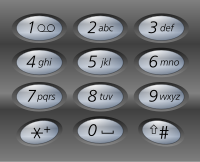
\includegraphics[width=150pt]{phone-keyboard.png}\\
\figcaption{Phone Keyboard}\label{fig:phone-keyboard}
\end{center}

\textbf{Input:}Digit string \code{"23"}

\textbf{Output:} \code{["ad", "ae", "af", "bd", "be", "bf", "cd", "ce", "cf"]}.

\textbf{Note:}
Although the above answer is in lexicographical order, your answer could be in any order you want.


\subsubsection{分析}
无


\subsection{递归}
\begin{Code}
// LeetCode, Letter Combinations of a Phone Number
// 时间复杂度O(3^n),空间复杂度O(n)
class Solution {
public:
    const vector<string> keyboard { " ", "", "abc", "def", // '0','1','2',...
            "ghi", "jkl", "mno", "pqrs", "tuv", "wxyz" };

    vector<string> letterCombinations (const string &digits) {
        vector<string> result;
        if (digits.empty()) return result;
        dfs(digits, 0, "", result);
        return result;
    }

    void dfs(const string &digits, size_t cur, string path,
            vector<string> &result) {
        if (cur == digits.size()) {
            result.push_back(path);
            return;
        }
        for (auto c : keyboard[digits[cur] - '0']) {
            dfs(digits, cur + 1, path + c, result);
        }
    }
};
\end{Code}


\subsection{迭代}
\begin{Code}
// LeetCode, Letter Combinations of a Phone Number
// 时间复杂度O(3^n),空间复杂度O(1)
class Solution {
public:
    const vector<string> keyboard { " ", "", "abc", "def", // '0','1','2',...
            "ghi", "jkl", "mno", "pqrs", "tuv", "wxyz" };

    vector<string> letterCombinations (const string &digits) {
        if (digits.empty()) return vector<string>();
        vector<string> result(1, "");
        for (auto d : digits) {
            const size_t n = result.size();
            const size_t m = keyboard[d - '0'].size();

            result.resize(n * m);
            for (size_t i = 0; i < m; ++i)
                copy(result.begin(), result.begin() + n, result.begin() + n * i);

            for (size_t i = 0; i < m; ++i) {
                auto begin = result.begin();
                for_each(begin + n * i, begin + n * (i+1), [&](string &s) {
                    s += keyboard[d - '0'][i];
                });
            }
        }
        return result;
    }
};
\end{Code}


\subsubsection{相关题目}
\begindot
\item 无
\myenddot
